\newpage
\appendix
\section{Annexes}

\subsection{Flow-sheet du plant}

\begin{figure}[!h]
\centering
   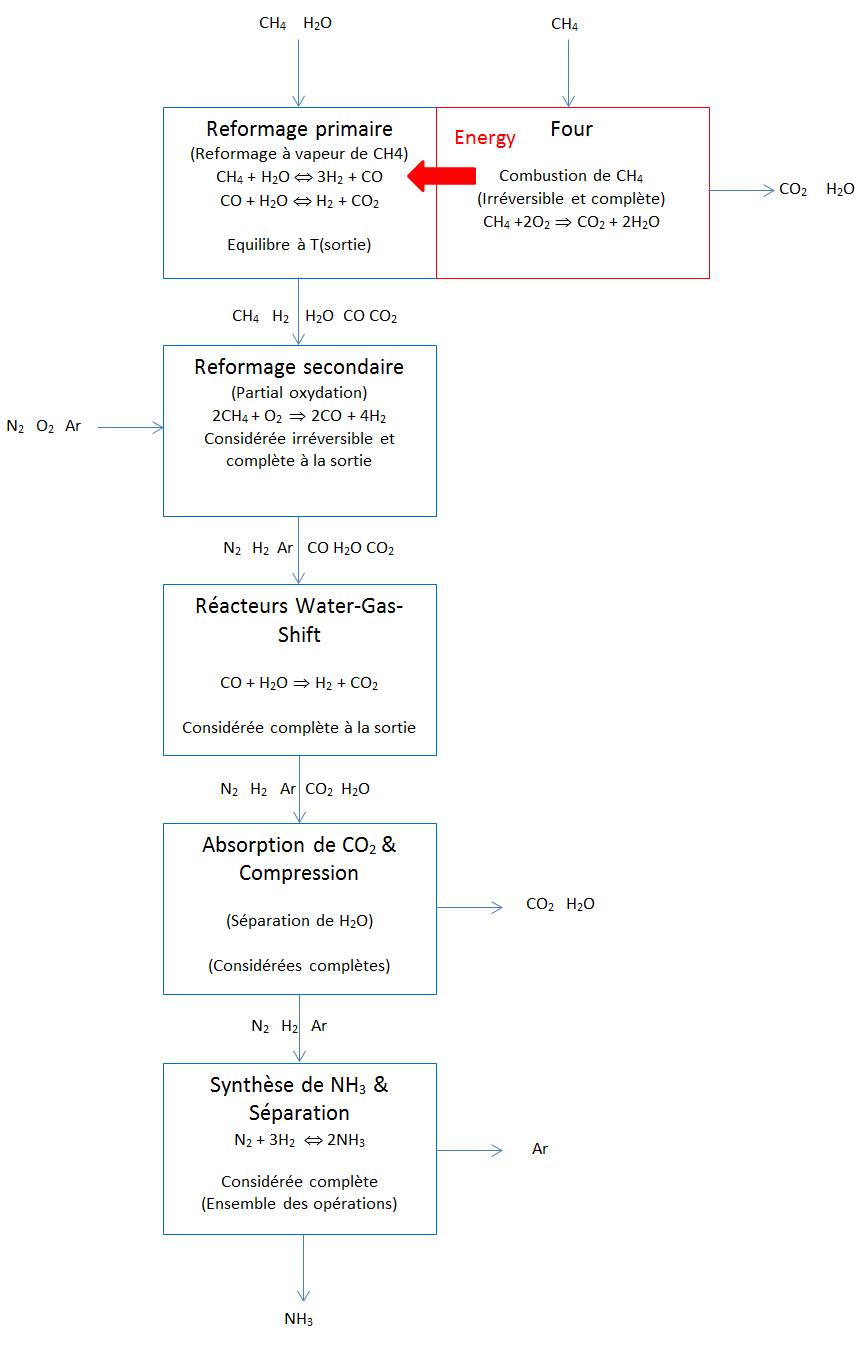
\includegraphics[scale=0.5]{flowsh.png}
\end{figure}

\newpage

\subsection{Données et constantes}
On connaît les valeurs de $\Delta H\degree (\unit{25}{\celsius})$ pour les éléments suivants:

\begin{itemize}
\item{\ce{CH_{4(g)}} $\Rightarrow \unit{-74.6}{\kilo\joule\per\mole}$}
\item{\ce{H_2O_{(g)}} $\Rightarrow \unit{-241.83}{\kilo\joule\per\mole}$}
\item{\ce{CO_{(g)}} $\Rightarrow \unit{-110.53}{\kilo\joule\per\mole}$}
\item{\ce{CO_{2(g)}} $\Rightarrow \unit{-393.51}{\kilo\joule\per\mole}$}
\item{\ce{H_{2(g)}} $\Rightarrow \unit{0}{\kilo\joule\per\mole}$}
\item{\ce{O_{2(g)}} $\Rightarrow \unit{0}{\kilo\joule\per\mole}$}
\end{itemize}

On connaît les constantes permettant d'utiliser la formule (\ref{eqref:capacite}):

\begin{table}[h]
\centering
\begin{tabular}{|c|c|c|c|c|c|c|}
\hline
\rule[-1ex]{0pt}{2.5ex} & A & B & C & D & E & G \\
\hline
\rule[-1ex]{0pt}{2.5ex} \ce{CH_{4(g)}} & -0.703 & 108.471 & -42.521 & 5.862 & 0.678 & 158.7163\\
\hline
\rule[-1ex]{0pt}{2.5ex} \ce{H_2O_{(g)}} & 30.092 & 6.832 & 6.793 & -2.534 & 0.082 & 223.3967\\
\hline
\rule[-1ex]{0pt}{2.5ex} \ce{CO_{(g)}} & 25.5675 & 6.0961 & 4.0546 & -2.6713 & 0.131 & 227.3665\\
\hline
\rule[-1ex]{0pt}{2.5ex} \ce{CO_{2(g)}} & 34.2244 & 41.044 & -23.5297 & 5.5352 & -0.129 & 228.2431\\
\hline
\rule[-1ex]{0pt}{2.5ex} \ce{H_{2(g)}} & 33.066 & -11.363 & 11.432 & -2.772 & -0.158 & 172.707974 \\
\hline
\end{tabular}
\caption{Tableau des constantes pour la formule (\ref{eqref:capacite})}
\label{tab:my_label}
\end{table}

\subsection{Code \textsc{MATLAB}}
Voici une fonction en \textsc{MATLAB} créée par nos soins, nous permettant de calculer l'enthalpie d'un élément à une certaine
température $T$, en fonction des différentes constantes utilisées dans la formule (\ref{eqref:capacite}).


\lstset{breaklines=true,frame=L,numbers=left}
\lstinputlisting[language=Matlab]{T(K)matlab.m}

